\subsection{The decomposition}\label{the-decomposition}

\Needspace*{12\baselineskip}\small\setlength{\tabcolsep}{3pt}\begin{longtable}[]{@{}
  >{\raggedright\arraybackslash}p{(\linewidth - 4\tabcolsep) * \real{0.3333}}
  >{\raggedright\arraybackslash}p{(\linewidth - 4\tabcolsep) * \real{0.3333}}
  >{\raggedright\arraybackslash}p{(\linewidth - 4\tabcolsep) * \real{0.3333}}@{}}
\caption{The four coalition states of the two-group game and the corresponding one-factor effects. Weighted Gini of the money metric on the raw household basis, with the female-primary reference for single-adult households. The fully common state is zero to the precision reported in the text: that is a tested property of the game, not an imposed constraint. A positive percentage in the last two rows is a rise in inequality.}\tabularnewline
\toprule\noalign{}
\begin{minipage}[b]{\linewidth}\raggedright
State
\end{minipage} & \begin{minipage}[b]{\linewidth}\raggedright
Single-adult
\end{minipage} & \begin{minipage}[b]{\linewidth}\raggedright
Couple
\end{minipage} \\
\midrule\noalign{}
\endfirsthead
\toprule\noalign{}
\begin{minipage}[b]{\linewidth}\raggedright
State
\end{minipage} & \begin{minipage}[b]{\linewidth}\raggedright
Single-adult
\end{minipage} & \begin{minipage}[b]{\linewidth}\raggedright
Couple
\end{minipage} \\
\midrule\noalign{}
\endhead
\bottomrule\noalign{}
\endlastfoot
Own preferences, own circumstances & 0.193596 & 0.132465 \\
Common preferences, own circumstances & 0.218795 & 0.129046 \\
Own preferences, common circumstances & 0.063459 & 0.009427 \\
Common preferences, common circumstances & 0.000000 & 0.000000 \\
\emph{Preferences equalized alone: change in the Gini (per cent)} & +13.02 & -2.58 \\
\emph{All other circumstances equalized alone: change (per cent)} & -67.22 & -92.88 \\
\end{longtable}

The four states are the coalition values of the two-group game. Reading them directly gives the one-factor effects. For single adults, equalizing preferences alone \emph{raises} the Gini by 13.0 per cent, from 0.193596 to 0.218795; equalizing all non-preference circumstances alone lowers it by 67.2 per cent. For couples, equalizing preferences alone lowers the Gini by 2.6 per cent and equalizing all other circumstances lowers it by 92.9. The fully common state is zero to 1.3e-15 in index units, which is a tested property of the game and not an imposed constraint.

\begin{figure}[H]
\centering
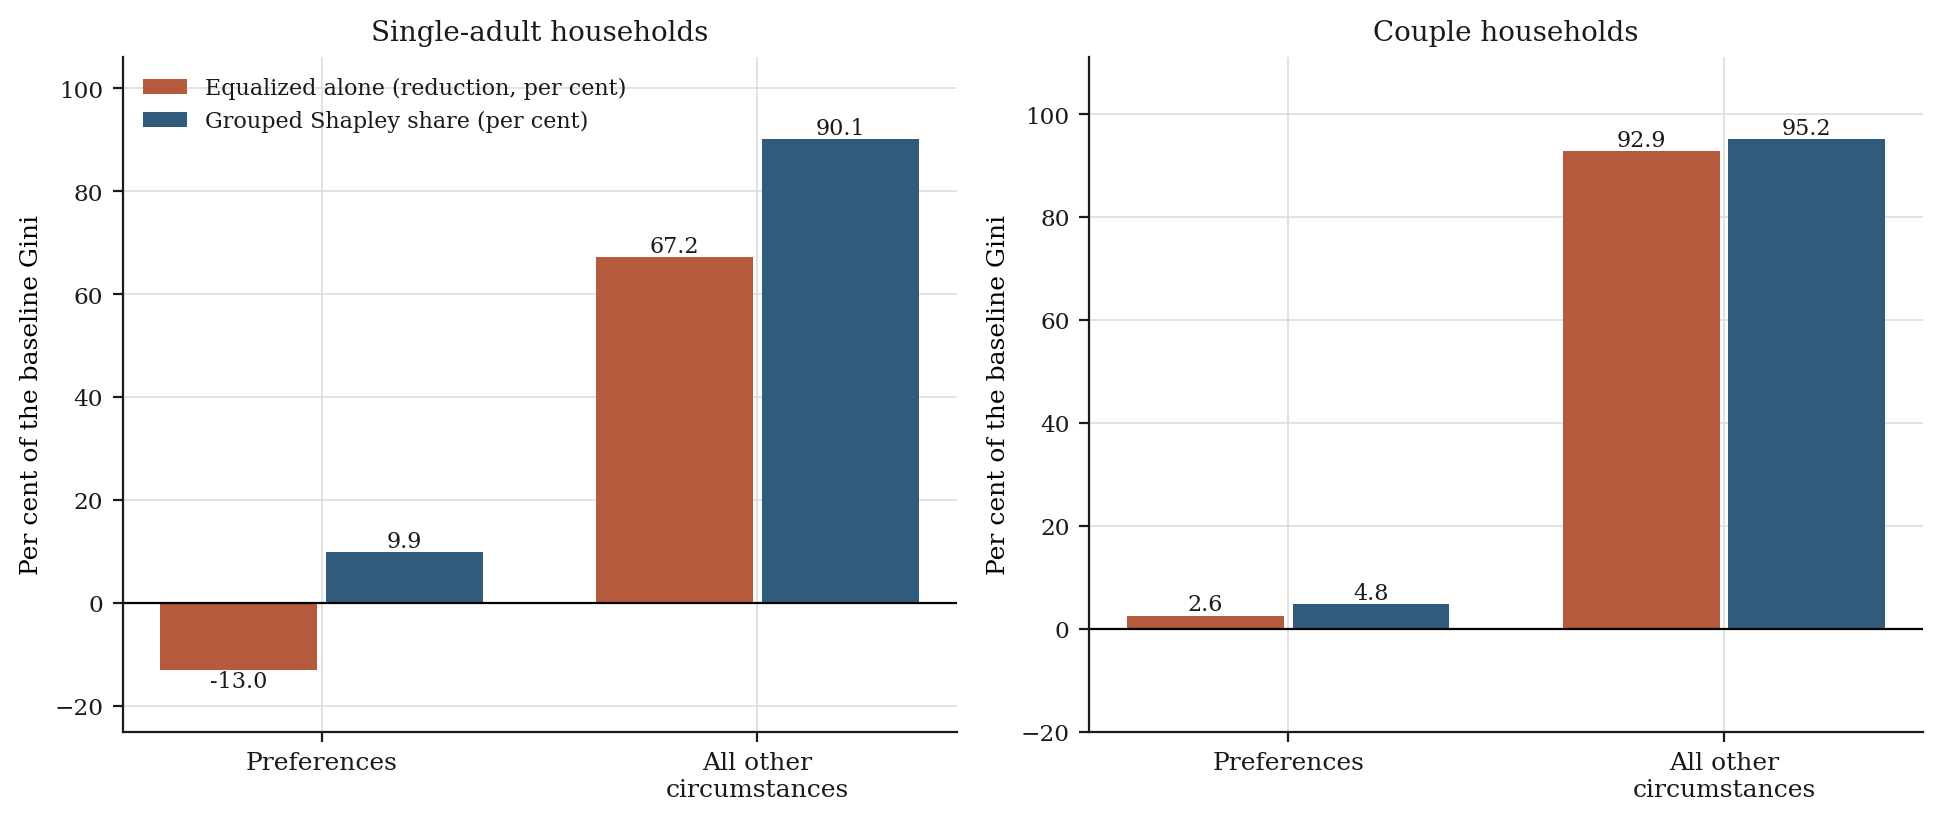
\includegraphics[width=0.95\linewidth,height=\textheight,keepaspectratio,alt={Equalizing one group alone against the grouped Shapley share. For single-adult households, equalizing preferences alone raises the Gini while the preference share is positive; the share averages marginal contributions over coalition orders and the one-factor effect does not.}]{figures/v5/figV04_one_factor_vs_shapley.png}
\caption{Equalizing one group alone against the grouped Shapley share. For single-adult households, equalizing preferences alone raises the Gini while the preference share is positive; the share averages marginal contributions over coalition orders and the one-factor effect does not.}
\end{figure}

The allocated shares are not those numbers. An allocated share is an average of marginal contributions over the orders in which coalitions can form; the one-factor effect is the contribution in exactly one order. For single adults the two even differ in sign, and the arithmetic of the game explains why. With four states and \(I_{11}=0\), the two-group closure gives

\[2\,C_P=I_{00}-I_{10}+I_{01}.\]

Since \(I_{01}\ge 0\) for a nonnegative index, a negative \(C_P\) forces \(I_{00}-I_{10}<0\), so a negative allocated share does imply that preference-only equalization raises inequality. The converse does not hold, and the single-adult Gini is the counterexample: \(C_P>0\) while \(I_{10}>I_{00}\). This is a consequence of the closure of \emph{this} exhaustive two-group game with a nonnegative index; it is not a general property of a Shapley allocation.

\Needspace*{12\baselineskip}\small\setlength{\tabcolsep}{3pt}\begin{longtable}[]{@{}
  >{\raggedright\arraybackslash}p{(\linewidth - 8\tabcolsep) * \real{0.2000}}
  >{\raggedright\arraybackslash}p{(\linewidth - 8\tabcolsep) * \real{0.2000}}
  >{\raggedright\arraybackslash}p{(\linewidth - 8\tabcolsep) * \real{0.2000}}
  >{\raggedright\arraybackslash}p{(\linewidth - 8\tabcolsep) * \real{0.2000}}
  >{\raggedright\arraybackslash}p{(\linewidth - 8\tabcolsep) * \real{0.2000}}@{}}
\caption{Grouped attribution of well-being inequality. Contributions in Gini points beside the share of the baseline Gini of the same population, per cent, with the 95 per cent cluster-robust parameter interval in brackets from 100 draws. Shares are taken against the baseline of the same population and are not comparable as levels across the two populations. The parameter interval and the RQMC integration band measure different things and are never combined; the integration band is reported separately in the text and in the figure. Resources and needs enter here as one component of the four-player game; its subdivision into non-labour resources and household composition is a nested attribution and has its own table.}\tabularnewline
\toprule\noalign{}
\begin{minipage}[b]{\linewidth}\raggedright
Component
\end{minipage} & \begin{minipage}[b]{\linewidth}\raggedright
Singles: Gini points
\end{minipage} & \begin{minipage}[b]{\linewidth}\raggedright
Singles: share {[}95 per cent{]}
\end{minipage} & \begin{minipage}[b]{\linewidth}\raggedright
Couples: Gini points
\end{minipage} & \begin{minipage}[b]{\linewidth}\raggedright
Couples: share {[}95 per cent{]}
\end{minipage} \\
\midrule\noalign{}
\endfirsthead
\toprule\noalign{}
\begin{minipage}[b]{\linewidth}\raggedright
Component
\end{minipage} & \begin{minipage}[b]{\linewidth}\raggedright
Singles: Gini points
\end{minipage} & \begin{minipage}[b]{\linewidth}\raggedright
Singles: share {[}95 per cent{]}
\end{minipage} & \begin{minipage}[b]{\linewidth}\raggedright
Couples: Gini points
\end{minipage} & \begin{minipage}[b]{\linewidth}\raggedright
Couples: share {[}95 per cent{]}
\end{minipage} \\
\midrule\noalign{}
\endhead
\bottomrule\noalign{}
\endlastfoot
Preferences & 0.019130 & 9.88 {[}6.1, 20.7{]} & 0.006423 & 4.85 {[}1.8, 9.7{]} \\
Job access & 0.095181 & 49.16 {[}36.0, 61.5{]} & 0.010901 & 8.23 {[}6.8, 11.6{]} \\
Earning opportunities & 0.013079 & 6.76 {[}2.7, 10.5{]} & 0.047313 & 35.72 {[}30.2, 38.3{]} \\
Market opportunities (A + B) & 0.108260 & 55.92 {[}43.0, 66.4{]} & 0.058215 & 43.95 {[}39.7, 47.7{]} \\
Resources and needs & 0.066206 & 34.20 {[}21.3, 41.2{]} & 0.067827 & 51.20 {[}46.4, 54.4{]} \\
All non-preference circumstances & 0.174466 & 90.12 & 0.126042 & 95.15 \\
\end{longtable}

\begin{figure}[H]
\centering
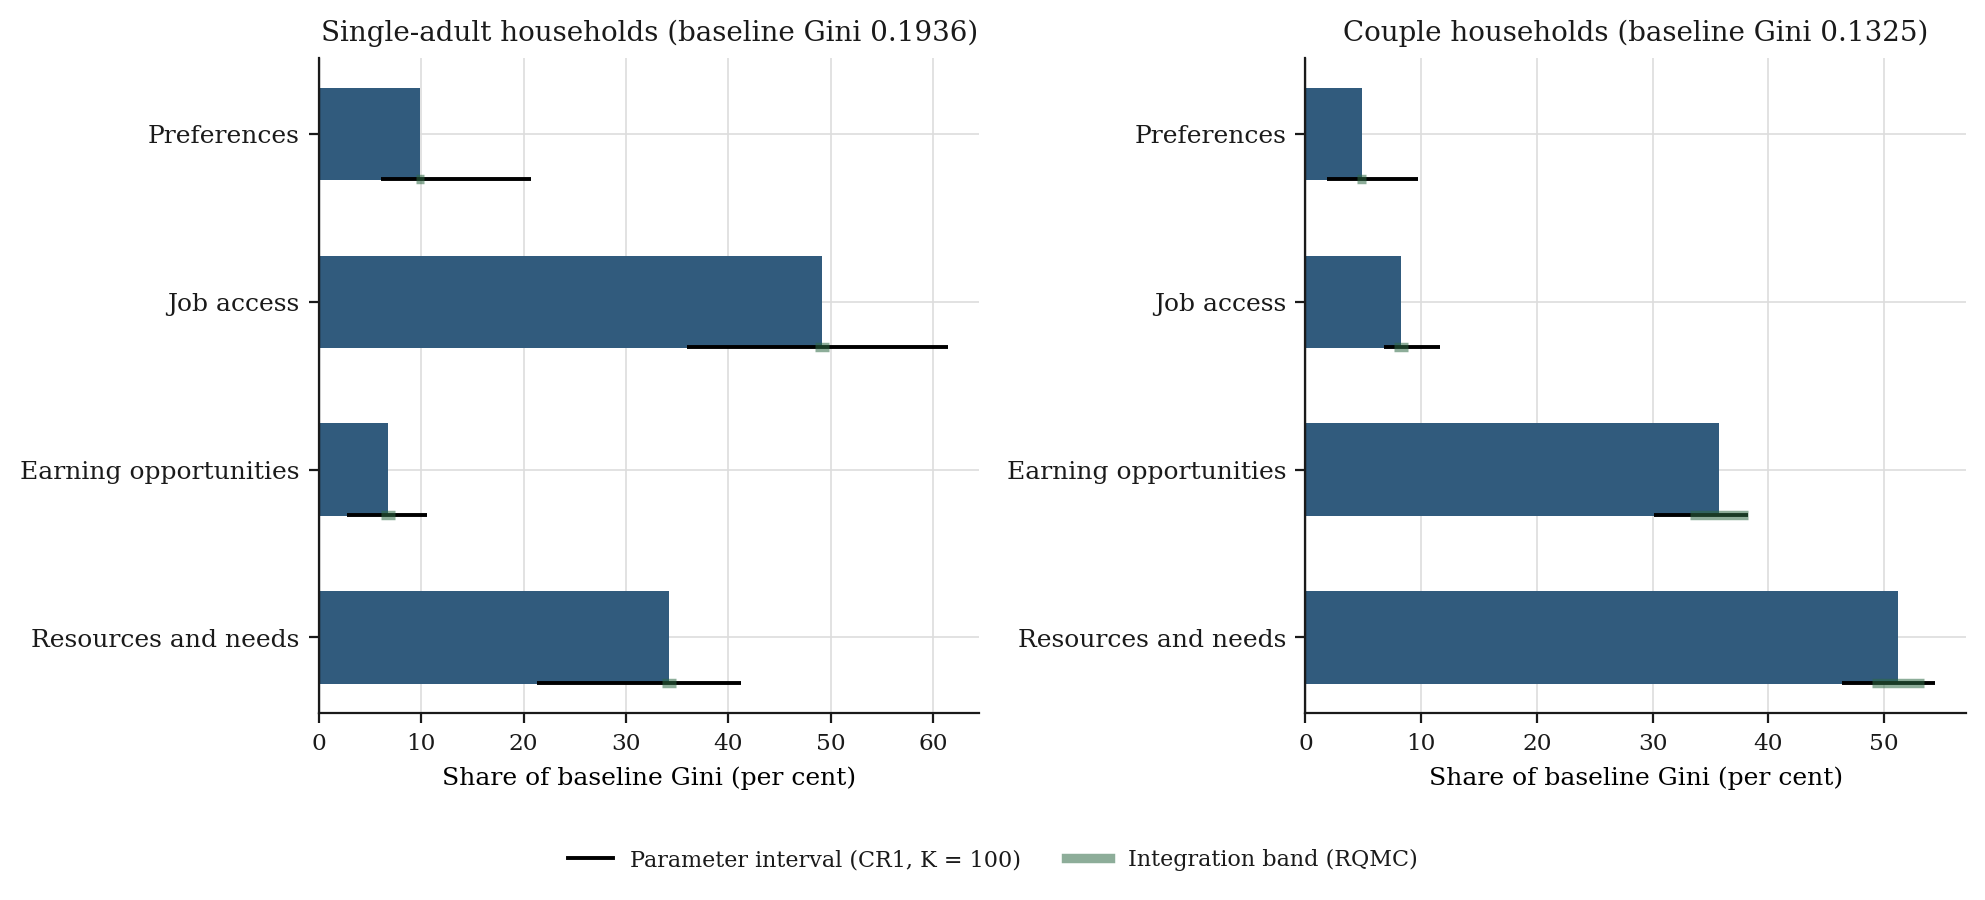
\includegraphics[width=0.95\linewidth,height=\textheight,keepaspectratio,alt={The grouped attribution, signed, in per cent of each population's own baseline Gini. The black bar is the 95 per cent cluster-robust parameter interval; the shaded bar is the RQMC integration band. They measure different things and are never combined.}]{figures/v5/figV03_signed_decomposition.png}
\caption{The grouped attribution, signed, in per cent of each population's own baseline Gini. The black bar is the 95 per cent cluster-robust parameter interval; the shaded bar is the RQMC integration band. They measure different things and are never combined.}
\end{figure}

The headline is the single-adult row. Labour-market opportunities, job access together with earning opportunities, carry 55.92 per cent of the inequality in the money metric; job access alone carries 49.16 per cent, with a 95 per cent cluster-robust parameter interval of 36.0 to 61.5 per cent. Preferences carry 9.88 per cent, earning opportunities 6.76 and household resources and needs 34.20. For couples the ordering is different: earning opportunities carry 35.72 per cent and resources and needs 51.20, while job access carries 8.23. Single adults are access-dominated on the labour-market side; couples are earnings- and resource-dominated, and access matters much less for them.

We report that contrast as a finding and attach no mechanism to it. A second earner is not automatically a buffer: two earnings streams do not mechanically produce less dispersion than one, since that depends on the dependence between them and on how resources pool. Establishing a mechanism would require a separately defined counterfactual, which we have not run. The contrast also cannot be assigned entirely to household type, because the two applications differ in their reference constructions as well; Section 6 reports the reference sensitivity.

The parameter interval and the integration band measure different things and are never combined. The integration band on the single-adult access share is 48.5 to 49.9 per cent, an order of magnitude narrower than the parameter interval, which is the expected ordering: the numerical integration is the accurate part and the parameters are the uncertain part.

The allocation is exhaustive. The maximum absolute top-level identity residual is 2.8e-17 in index units and the nested residual 5.6e-17. That is a computational validation of the accounting for the declared game. It does not validate the identification of the model or the normative content of the operators.

